\subsection{Ce qu'on entend par régularité locale}
\label{sec:ce-qu-on-entend-par-reguarite-locale}

Longtemps, il était cru que les fonctions continues étaient dérivables presque partout. C'est notamment Weierstrass qui a démontré qu'il existe des fonctions continues partout mais dérivable nulle part. Poincaré notamment disait de tels objets qu'ils n'existaient que pour contredire le travail des pères.
Cependant, des objets manipulés tous les jours comme le monde de la finance notamment traitent des processus qui sont fondamentalement irréguliers
%
\footnote{les fonctions dérivables nulle part sont même denses dans les fonctions continues pour la topologie de la convergence uniforme~\cite{gourdon2020maths-dense-non-deriv}. A epsilon près on rencontre toujours une fonction dérivable nulle part lorsque l'on considère la distance maximale réalisée entre deux fonctions continues sur leur support $I$...}
%
(au point de vue de l'analyse, où l'on traite souvent des fonctions au moins dérivables). Il est donc important de pouvoir quantifier la régularité d'une fonction de façon plus fine que le nombre de dérivées qu'elle possède.

Nous allons repasser rapidement en revue les différents concepts de régularité pour mettre l'emphase sur ce que l'on considère comme régularité locale.

Afin de savoir à quel niveau de régularité nous souhaitons estimer, il est important de garder en tête un ordre de différents niveaux de régularité résumé par les relations suivantes :

$$\textsf{Lipschitz} \implies \textsf{Hölder} \implies \underbracket[0.187ex]{\colorize{\textsf{Localement Hölder}}}_{\textsf{ce qui nous intéresse}} \implies \textsf{Uniformément continue} \implies \textsf{Continue}$$

Afin de mieux discerner ce que chaque propriété signifie, et quelles sont les différences entre chaque niveau de régularité, il est conseillé de se rappeler rapidement les définitions de ces propriétés disponibles en annexe \ref{annexe:regularite-def}.

\question{
	\smallskip\centering
	Pourquoi se concentrer sur des processus localement Hölder ?
}

La nature des phénomènes rencontrés dans la vie réelle est souvent complexe. Influencés par de nombreux phénomènes, certains d'entre eux sont, comme mentionnés précédemment, irréguliers. C'est notamment le cas des courbes de charge électriques, qui dépendent de multitudes de phénomènes physiques ou comportementaux, dont on peut attendre une certaine régularité, mais qui ne sont pas nécessairement uniformes tant sur leur niveau régularité que l'intervalle de temps sur lequel ils ont une influence. On pourrait par exemple attendre une différence de régularité de la production électrique en plein été (soleil et température stables \ldots) comparé au mois de mars (plus grande instabilité des conditions climatiques).

De plus, les fonctions Hölderiennes représentent une classe suffisamment large de fonctions.
L'espace de fonctions sur lequel on travail est donc devrait être en pratique suffisamment grand pour inclure l'ensemble des processus qui nous intéressent. Enfin les fonctions que le praticien sera amené à manipuler seront des fonctions d'un intervalle dans $\mathds R$, qui lorsque continues sont automatiquement uniformément continues en vertu du théorème de Heine. Il est donc naturel de se concentrer sur des fonctions localement Hölderiennes. \footnote{Afin de ne pas alourdir l'essence du propos, une simplification par rapport à l'article de MPV~\cite{maissoro-SmoothnessFTSweakDep} a été faite, si le lecteur souhaite aller dans le détail, il est possible de se référer à l'Annexe \ref{annexe:regularite-locale}.}



\subsection{Modèle considéré}

On dispose désormais de tous les ingrédients pour expliciter le modèle considéré pendant l'ensemble du stage :

% \begin{figure}[H]
% 	\noindent\begin{tabularx}{\textwidth}{XcX}
% 		\toprule
% 		\textbf{Nom}                                                                                   & \textbf{Objet} & \textbf{Définition}                                                                \\
% 		\midrule
% 		Nombre de Burn-in pour atteindre la stationnarité du $\operatorname{FAR}(1)$                   & $B$            & $\in \mathds N^*$                                                                  \\
% 		Nombre de courbes gardées après le Burn-in                                                     & $N$            & $\in \mathds N^*$                                                                  \\

% 		Ensemble de points $t \in \mathcal T$ où l'on génère le mouvement Brownien multi-fractionnaire & $T$            & $T = T_{\textsf{estim.reg}(\Delta)} \bigcup T_{\int} \bigcup T_{\textsf{observé}}$ \\

% 		\bottomrule
% 	\end{tabularx}
% 	\caption{Notations des objets utilisés pour les algorithmes de simulation}
% 	\label{tab:algo_notations}
% \end{figure}


\begin{table}[H]
\centering
	\noindent\begin{tabularx}{\textwidth}{XcX}
		\toprule
		\textbf{Nom}                                 & \textbf{Objet}                              & \textbf{Définition}                                                                                                \\
		\midrule
		Régularité : constante locale                & $L$                                         & $: \func{[0,1]}{\mathds R}{t}{L_t}$                                                                                \\
		Régularité : puissance locale de l'incrément & $H$                                         & $: \func{[0,1]}{[0,1]}{t}{H_t}$                                                                                    \\
		donnée fonctionnelle                         & $X$                                         & $\in \VA{ \mathds L^2 \cap \mathcal H(H, L) }$                                                                     \\
		$N$-échantillon de la loi de $X$             & $(X_n)_{n \in \intervaleint 1 N}$           & $X_n \sim X$                                                                                                       \\
		\midrule
		Nombre de points sur la trajectoire de $X_n$ & $M_n$                                       & $\sim \mathcal P(\lambda)$                                                                                         \\
		Temps observés                               & $\bigl(T_n[m]\bigr)_{m \in 1:M_n}$          & $\sim \mathcal U( [0,1] )^{\otimes M_n}$                                                                           \\
		\midrule
		écart type de l'erreur                       & $\sigma$                                    & $\in \mathds R_+^*$                                                                                                \\
		erreur                                       & $\eta$                                      & $\sim \mathcal N(0, \sigma^2)$                                                                                     \\
		% $ Uncomment to create two tables
% 		\bottomrule
% 		\end{tabularx}
% 		\end{table}
% \begin{table}[H]
% \centering
% 		\noindent\begin{tabularx}{\textwidth}{XcX}
% 		\toprule
% 		\textbf{Nom}                       & \textbf{Objet}                              & \textbf{Définition}                                                                                                \\
		% $ Uncomment to create two tables
		\midrule
		noyau de l'opérateur intégral                & $\beta$                                     & $\in \mathds L^2([0,1])$                                                                                           \\
		relation auto-régressive intégrale           & $\phi$                                      & $: \func{\mathds L^2([0,1], \mathds R)}{\mathds L^2([0,1], \mathds R)}{f}{\int_0^1 \beta(u, \cdot \, )f(u) \, du}$ \\
		FAR(1)                                       & $X_{n+1}$                                   & $= \phi( X_n )+ \xi_{n+1}$                                                                                         \\
		\midrule
		observation                                  & $Y_n[m]$                                    & $= X_n( T_n[m] ) + \eta_{n}[m] $                                                                                \\
		observation                                  & $\bigl( T_n[m] \, , \, Y_n[m] \bigr)_{n,m}$ & $\in [0,1] \times \mathds R$                                                                                       \\
		\bottomrule
	\end{tabularx}
	\caption{Tableau récapitulatif du modèle considéré}
	\label{tab:model}
\end{table}

% \footnote{$L_t$ dépend du voisinage considéré ($J_\Delta(t)$) mais constate sur celui-ci}

\subsection{Deux méthodes d'obtention de la régularité locale des trajectoires}
\label{sec:deux_methodes_estim}

Il existe deux méthodes différentes pour estimer la régularité des trajectoires. Si la clé des deux méthodes pour extraire la régularité locale est le théorème de continuité de Kolmogorov\footnote{$cf$ Annexe \ref{annexe:continuite_kolmogorov}}, les deux méthodes diffèrent par les points $t \in \mathcal T$ considérés dans l'estimation des accroissements quadratiques $\esperance{ \vert X(u) - X(v) \vert^2 }$ utilisés pour l'estimation de la régularité locale.

La méthode de Golovkine et al. ~\cite[pages : 7—9]{golovkineRegularityOnlineEstimationNoisyCurve} n'utilise que les points observés, et construit un estimateur des incréments quadratiques à base de statistique d'ordre.

\begin{equation*}
	\theta( T_{(l)}, T_{(k)}) = \esperance{ \left| X( T_{(l)}) - X(T_{(k)}) \right|^2 }  \begin{array}{ccc}
		 & \quad \underset {\textsf{LGN}} \approx
		 & \boxed{\frac 1 {N} \sum\limits_{n=1}^N \left| \statrang Y n {2k-1} \statrang Y n k \right|^2 \isdef \hat \theta_k}
		\\
		 & \, \underset {+ \mathcal C^0 Kol.} {\overset {\textsf{Hölder}} \approx}
		 & L_{t_0} \esperance{| \ordered T l - \ordered T k |^{2H_{t_0}}}
	\end{array}
\end{equation*}

et on obtient ainsi l'estimateur suivant :

\begin{equation*}
	\widehat H_{t}(k) =
	\begin{cases} \displaystyle\frac{\log\left( \hat \theta_{4k-3} - \hat \theta_{2k-1}  \right) - \log \left(  \hat\theta_{2k-1} - \hat \theta_k \right)}{2\log 2}
		 & \hat \theta_{4k-3} > \hat \theta_{2k-1} > \hat \theta_{k}
		\\
		1
		 & \textsf{sinon}
	\end{cases}
\end{equation*}

\info{Cette méthode peut s'avérer spécifiquement utile lorsque l'on traite un flux de données, car l'arrivée de nouvelles données ne nécessite pas spécifiquement de recalculer les incréments quadratiques sur l'ensemble des points observés. }

L'autre méthode proposée dans les articles ~\cite{golovkine2021adaptive,maissoro-SmoothnessFTSweakDep}, elle se base sur l'utilisation de points non observés, inférés par lissage des courbes, à une distance $\Delta / 2$ les uns des autres pour estimer les incréments quadratiques. Cette dernière méthode implique le choix d'un hyper-paramètre lors de l'estimation $\Delta$ et pourrait être sensible à la qualité du lissage de la courbe. Etant donné que l'objectif de la détermination de la régularité locale est de pouvoir faire un lissage à noyaux adaptatif en fonction de l'objet que l'on souhaite estimer, on appelle le lissage effectué pour estimer la régularité \og pré-lissage \fg.

\smallskip

On se donne un $\Delta \in \, ] \, 0,1 \,[$, arbitraire pour le moment, comme diamètre de l'intervalle $J_\Delta$ que l'on considère pour évaluer la régularité en $t_0$.

\noindent Il est naturel de définir les points d'estimation de la régularité de la façon suivante :

\begin{minipage}{0.5\textwidth}
	\begin{align*}
		t_1 & \isdef t_0 - \frac \Delta 2 \\
		t_2 & \isdef t_0                  \\
		t_3 & \isdef t_0 + \frac \Delta 2
	\end{align*}
\end{minipage}
\hfill
\begin{minipage}{0.5\textwidth}
	\begin{equation*}
		J_\Delta = [t_1, t_3]
	\end{equation*}

	\begin{center}
		avec $t_0$ le point en lequel on souhaite estimer la régularité.
	\end{center}
\end{minipage}


% https://tex.stackexchange.com/questions/156993/plotting-weierstrass-function
\begin{figure}[H]
	\centering
	\begin{minipage}{0.45\linewidth}
		\scalebox{0.885}{
			\begin{tikzpicture}
	\pgfmathsetmacro{\pgfdeltavalue}{0.25}
	\pgfmathsetmacro{\pgftvalue}{0.4}
	\pgfmathsetmacro{\pgfarrowheight}{-0.25}
	\pgfmathsetmacro{\pgfarrowfrom}{\pgftvalue - \pgfdeltavalue/2}
	\pgfmathsetmacro{\pgfarrowto}{\pgftvalue + \pgfdeltavalue/2}
	\begin{axis}[axis lines=middle,
			xmin=0, xmax=1,
			ymin=-0.4, ymax=0.4,
			axis equal image,
			ytick=\empty,
			xtick=\empty,
			legend style={at={(0.5,-0.15)},anchor=north},
			legend entries={X, Point d'estimation de la régularité locale}
		]
		\addplot [flatuicolors_green, samples=800, domain=0:1.1] {weierstrass(2*x,2,15)};

		\addplot [flatuicolors_red_light, mark=*, only marks] coordinates {(\pgftvalue, {weierstrass(2*\pgftvalue,2,15)})};
		\addplot [flatuicolors_imperial, mark=*, only marks] coordinates {(\pgftvalue - \pgfdeltavalue/2, {weierstrass(2*(\pgftvalue - \pgfdeltavalue/2),2,15)})};
		\addplot [flatuicolors_imperial, mark=*, only marks] coordinates {(\pgftvalue + \pgfdeltavalue/2, {weierstrass(2*( \pgftvalue + \pgfdeltavalue/2 ),2,15)})};

		\addplot[color=flatuicolors_imperial,mark=none, thick, dashed] (\pgftvalue + \pgfdeltavalue/2,x);
		\addplot[color=flatuicolors_imperial,mark=none, thick, dashed] (\pgftvalue - \pgfdeltavalue/2,x);
		\addplot[color=flatuicolors_imperial,mark=none, thick, dashed] (\pgftvalue,x);

		\draw[color=white, fill=white] (\pgftvalue - 0.005, \pgfarrowheight - 0.05 - 0.025) rectangle (\pgftvalue + 0.005, \pgfarrowheight - 0.05 + 0.025);
		\node at (axis cs: \pgftvalue, \pgfarrowheight - 0.05) {$\colorize[flatuicolors_aqua]{ \mathbf \Delta}$};

		\draw[flatuicolors_aqua, ->] (axis cs:\pgfarrowfrom, \pgfarrowheight) -- (axis cs: \pgfarrowto, \pgfarrowheight);
		\draw[flatuicolors_aqua, <-] (axis cs:\pgfarrowfrom, \pgfarrowheight) -- (axis cs: \pgfarrowto, \pgfarrowheight);

		\draw[color=white, fill=white] (\pgftvalue - 0.05, -0.06) rectangle (\pgftvalue + 0.05,-0.005);
		\node at (axis cs: \pgftvalue,  -0.03 ) {$\colorize[flatuicolors_imperial]{ t_2}$};
		\draw[color=white, fill=white] (\pgftvalue - \pgfdeltavalue/2 - 0.05, -0.06) rectangle (\pgftvalue - \pgfdeltavalue/2 + 0.05,-0.005);
		\node at (axis cs: \pgftvalue - \pgfdeltavalue/2 -0.01,- 0.03) {$\colorize[flatuicolors_imperial]{ t_1}$};
		\draw[color=white, fill=white] (\pgftvalue + \pgfdeltavalue/2 - 0.005, 0.005) rectangle (\pgftvalue + \pgfdeltavalue/2 + 0.005, 0.08);
		\node at (axis cs: \pgftvalue + \pgfdeltavalue/2, 0.04 ) {$\colorize[flatuicolors_imperial]{ t_3}$};

	\end{axis}

\end{tikzpicture}

		}
	\end{minipage}
	\hfill
	\begin{minipage}{0.45\linewidth}
		\scalebox{0.885}{
			\begin{tikzpicture}
	\pgfmathsetmacro{\pgfdeltavalue}{0.25}
	\pgfmathsetmacro{\pgftvalue}{0.15}
	\pgfmathsetmacro{\pgfarrowheight}{-0.25}
	\pgfmathsetmacro{\pgfarrowfrom}{\pgftvalue - \pgfdeltavalue/2}
	\pgfmathsetmacro{\pgfarrowto}{\pgftvalue + \pgfdeltavalue/2}
	\begin{axis}[axis lines=middle,
			xmin=0, xmax=1,
			ymin=-0.4, ymax=0.4,
			axis equal image,
			ytick=\empty,
			xtick=\empty,
			legend style={at={(0.5,-0.15)},anchor=north},
			legend entries={X, Point d'estimation de la régularité locale},
		]
		\addplot [flatuicolors_green, samples=800, domain=0:1.1] {weierstrass(2*x,2,15)};

		\addplot [flatuicolors_red_light, mark=*, only marks] coordinates {(\pgftvalue - \pgfdeltavalue/2, {weierstrass(2*(\pgftvalue - \pgfdeltavalue/2),2,15)})};
		\addplot [flatuicolors_imperial, mark=*, only marks] coordinates {(\pgftvalue, {weierstrass(2*\pgftvalue,2,15)})};
		\addplot [flatuicolors_imperial, mark=*, only marks] coordinates {(\pgftvalue + \pgfdeltavalue/2, {weierstrass(2*( \pgftvalue + \pgfdeltavalue/2 ),2,15)})};

		\addplot[color=flatuicolors_imperial,mark=none, thick, dashed] (\pgftvalue + \pgfdeltavalue/2,x);
		\addplot[color=flatuicolors_imperial,mark=none, thick, dashed] (\pgftvalue - \pgfdeltavalue/2,x);
		\addplot[color=flatuicolors_imperial,mark=none, thick, dashed] (\pgftvalue,x);

		\draw[color=white, fill=white] (\pgftvalue - 0.005, \pgfarrowheight - 0.05 - 0.025) rectangle (\pgftvalue + 0.005, \pgfarrowheight - 0.05 + 0.025);
		\node at (axis cs: \pgftvalue, \pgfarrowheight - 0.05) {$\colorize[flatuicolors_aqua]{ \mathbf \Delta}$};

		\draw[flatuicolors_aqua, ->] (axis cs:\pgfarrowfrom, \pgfarrowheight) -- (axis cs: \pgfarrowto, \pgfarrowheight);
		\draw[flatuicolors_aqua, <-] (axis cs:\pgfarrowfrom, \pgfarrowheight) -- (axis cs: \pgfarrowto, \pgfarrowheight);

		\draw[color=white, fill=white] (\pgftvalue - 0.05, -0.06) rectangle (\pgftvalue + 0.05,-0.005);
		\node at (axis cs: \pgftvalue,  -0.03 ) {$\colorize[flatuicolors_imperial]{ t_1}$};
		\draw[color=white, fill=white] (\pgftvalue - \pgfdeltavalue/2 - 0.005, -0.06) rectangle (\pgftvalue - \pgfdeltavalue/2 + 0.005,-0.005);
		\node at (axis cs: \pgftvalue - \pgfdeltavalue/2,- 0.03) {$\colorize[flatuicolors_imperial]{ t_2}$};
		\draw[color=white, fill=white] (\pgftvalue + \pgfdeltavalue/2 - 0.005, 0.005) rectangle (\pgftvalue + \pgfdeltavalue/2 + 0.005, 0.08);
		\node at (axis cs: \pgftvalue + \pgfdeltavalue/2, 0.04 ) {$\colorize[flatuicolors_imperial]{ t_3}$};

	\end{axis}

\end{tikzpicture}

		}
	\end{minipage}
	% \caption{Illustration de la méthode \og prélissage \fg pour estimer la régularité locale.}
	\label{fig:delta_method_example}
	\caption{Exemple de courbe dont on souhaiterait déterminer la régularité locale, et visualisation de $J_\Delta$ : estimation intérieure / au bord}
\end{figure}

\info{
	\begin{rem}
		Rien n'empêche dans la théorie d'avoir les points $t_1, t_2, t3$ non ordonnés dans le temps, mais dans la pratique, on considère naturellement que $t_1 < t_2 < t_3$. Mais cet ordre n'est pas obligatoire.
		Ainsi aux bords, si l'on souhaite estimer la régularité au point $t_0$ tel que la définition précédente nous donne un point $t_1$ en dehors de $[0,1]$, on peut tout à fait à la place considérer :

		\begin{minipage}{0.5\linewidth}
			$$t_2 \isdef t_0$$
			$$t_1 \isdef t_0 + \frac \Delta 2$$
			$$t_3 \isdef t_0 + \Delta$$
		\end{minipage}
		\begin{minipage}{0.5\linewidth}
			\centering
			on pourra se référer à la 2$^e$ image de la figure \ref{fig:delta_method_example}
		\end{minipage}
	\end{rem}
}

\info{
	Le point $t_0$, où l'on souhaite estimer la régularité, étant dans la majorité des cas le point central de l'intervalle $J_\Delta$ considéré; il sera à présent mentionné comme le point $t_2$. Il s'agit à la fois d'un moyen de se rappeler dans les formules suivantes que l'on considère le point central de l'intervalle $J_\Delta$ et d'être au plus proche des noms de variables considérés dans l'implémentation.
}

alors on approche $\theta (t_1,t_3) = \esperance{ \left| X(t_3) - X(t_1) \right|^2 }$ par :

\begin{equation*}
	\tilde \theta(t_1,t_3) = \frac 1 N \sum\limits_{n=1}^N \left| X_n\bigl(t_3\bigr) - X_n\bigl(t_1\bigr) \right|^2
\end{equation*}

\noindent qui n'est pas observable, étant donné qu'il n'est pas garanti d'observer $X(t_1)$ et $X(t_3)$, et qu'il faut donc lisser dans un premier temps les courbes pour pouvoir évaluer $X$ en $t_1$ et $t_3$. L'estimateur que l'on considère est donc une approximation de $\tilde \theta_{13}$, et est défini par :

\begin{equation*}
	\hat \theta(t_1,t_3) = \frac 1 N \sum\limits_{n=1}^N \left| \widehat X_n(t_3) - \widehat X_n(t_1) \right|^2
\end{equation*}

où $\hat X$ est la courbe lisssée à partir des observations :

\begin{equation*}
	( T_n[ m \,], Y_n[ m \,] )_{{n \in 1:N} \; , \; {m \in 1:M_n}}
\end{equation*}

avec :

\begin{itemize}
	\item $N$ : Nombre de courbes observées
	\item $M_n$ : Nombre de points observés (aléatoire) sur la trajectoire de $X_n$
\end{itemize}

Les estimateurs des paramètres de régularité sont alors les suivants ~\cite{maissoro-SmoothnessFTSweakDep}:

\begin{definition}[estimateurs des paramètres de régularité]
	.

	\begin{minipage}{0.5\textwidth}
		\begin{align*}
			\hat H_{t_2} & = \frac{ \log \hat \theta(t_1, t_3) - \log \hat \theta(t_1, t_2) }{2 \log 2}
			\\
			\textbf{ou}
			\\
			\hat H_{t_2} & = \frac{ \log \hat \theta(t_1, t_3) - \log \hat \theta(t_2, t_3) }{2 \log 2}
		\end{align*}
	\end{minipage}
	\begin{minipage}{0.5\textwidth}
		\begin{align*}
			\widehat L_{t_2} & = \frac{\widehat \theta(t_1, t_3)}{\Delta^{2 \widehat H_{t_2}}}
			\\ &\underset{ou}= \frac{\widehat \theta(t_1, t_2)}{\Delta^{2 \widehat H_{t_2}}}
			\\ &\underset{ou}= \frac{\widehat \theta(t_2, t_3)}{\Delta^{2 \widehat H_{t_2}}}
		\end{align*}
	\end{minipage}
\end{definition}


\subsection{Prélissage}
\label{sec:regloc-prelissage}

Comme mentionné précédemment, l'estimation de la régularité locale nécessite l'évaluation de notre processus observé $X$ en 3 points. Il est possible de ne pas observer ces points, qui sont de plus bruités dû au sampling de $X$. C'est pourquoi nous décidons de lisser les courbes comme \og pré-lissage \fg pour pouvoir estimer la régularité locale.

\question{
	\smallskip\centering
	Pourquoi parle-t-on de \textbf{pré}-lissage ? Le but de considérer la régularité n'était-il pas justement de l'utiliser dans le lissage des trajectoires ? Lisser avant même d'estimer la régularité n'est-il pas contre-productif ?
}

L'objectif de l'obtention des paramètres de régularité des trajectoires est de pouvoir effectuer un lissage de ces trajectoires qui préserve les irrégularités fondamentales du processus dont elles sont issues, tout en éliminant le bruit. Les paramètres de régularité sont donc dans un premier temps estimés en utilisant des trajectoires lissées puis utilisés pour effectuer un \textbf{nouveau lissage} à noyaux en utilisant, cette-fois, une fenêtre de lissage appropriée qui dépend de ces paramètres de régularité.

En d'autres termes, le pré lissage utilise un lissage à noyaux tel que la fenêtre de lissage cross-validée nous donne :


\begin{equation*}
	h^{*[\textsf{cv}]}_{\textsf{pre}} \textsf{ estimateur de } h^*_{\mathcal R_{\textsf{quadr}}}(t) = \grandop{ \lambda^{- \frac 1 {2  H_t + 1}}}
\end{equation*}

à partir duquel on peut lisser les courbes observées $( T_i^{[n]}, Y_i^{[n]} )_{n \in 1:N, i \in 1:M_n}$ pour estimer la régularité locale $H_t$. On peut désormais obtenir la fenêtre de lissage adaptée à la quantité que l'on souhaite estimer :

\begin{equation*}
	h_\mu^*(t) = \argmin\limits_h \mathcal R_\mu(\underset {\rightarrow H_t \;, \; L_t \; , \; \mathcal W_t}{\underbrace{\quad t \quad}_{\textsf{Régularité, sparsity, ...}}}, h)
\end{equation*}



\bigskip

Le coeur de ce stage est la détermination du comportement dé l'hyper-paramètre $\Delta$, diamètre de l'intervalle que l'on considère dans lequel on vient prendre la valeur de notre processus en 3 points régulièrement espacés. MPV affirme déjà que pour un $\Delta$ donné, on a bien la convergence ponctuelle des estimateurs. Ces points ne sont pas nécessairement observés, et on va donc effectuer un pré-lissage. \cite{maissoro-SmoothnessFTSweakDep}

\smallskip

Toutefois, le praticien est en droit de se demander quel $\Delta$ explicitement choisir ? Est ce qu'il y a une procédure simple pour déterminer la valeur optimale de $\Delta$ qu'il faut choisir pour obtenir un biais le plus petit possible pour l'estimation des paramètres de régularité ?

\question{ la méthode de pré-lissage a-t-elle une importance ? SI oui, laquelle faut-il choisir ?}

C'est pourquoi nous allons établir une première heuristique avant d'aborder le comportement du $\Delta$ :

\subsubsection{pré-lissage Spline}

Le lissage spline est certainement une des méthodes de lissage les plus répandues de par sa simplicité d'implémentation. De plus la détermination des hyper-paramètres de lissage via la méthode de GCV permet de déterminer une approximation de base optimale à un coût computationnel relativement faible. Un des plus grands avantages du lissage B-Spline est l'obtention d'une base de fonctions, qui permet à coût de stockage faible de pouvoir prédire des points non observés. Une fois la base déterminée, il ne reste plus qu'à prédire les points non observés en utilisant la base de fonctions et les coefficients de la décomposition de la courbe sur cette base.

\bigskip

On rappelle que l'utilisation de Splines comme méthode de lissage nécessite tout de même de faire des choix : elle est sensible aux nombre de noeuds et leur emplacement. Il est donc nécessaire de les déterminer par validation croisée. Une méthode fréquemment utilisée est d'utiliser un nombre de noeuds $\mathcal k$ égal au nombre d'observations, et de les placer aux points d'observations. Puis on utilise des splines pénalisées sur leur dérivée seconde ( $L = L_{quad} + \lambda \displaystyle\int_0^1 f''(u) du$ ) et on détermine le paramètre de pénalisation par validation croisée afin de s'affranchir du choix du nombre de noeuds et de leur emplacement. La validation croisée sur la pénalisation est supposée compenser ce choix. Il s'agit de la méthode qui a été utilisée dans le cadre de ce stage, car très populaire et simple à mettre en place.

Il est à noter qu'une autre méthode de lissage spline est de déterminer le nombre de noeuds $\mathcal k$ par validation croisée, et de placer les points de façon uniforme sur les quantiles de la distribution des observations. Ce qui ne sera pas utilisé dans le cadre de ce stage.

\bigskip

En effectuant un pré-lissage de splines cubiques naturelles sur une courbe Höldérienne, on ne s'attend pas à obtenir de bonnes performances sur l'estimation de la régularité locale. En effet les courbes splines sont par construction de classe $\mathcal C^2$ (fonctions polynômiales $\mathcal C ^\infty$ avec des raccordements $\mathcal C^2$), et la courbe lissée écrasera complétement l'information de régularité. Même si il s'agit de ce que l'on souhaite obtenir et qu'on ne connait pas encore la régularité, il est raisonnable de penser qu'être précautionneux dans le choix de la technique de lissage de telle façon à être le plus proche de la régularité d'une fonction qui pourrait potentiellement ne même pas être dérivable est une bonne idée.



\subsubsection{pré-lissage à noyaux}

Considérer un lissage non paramétrique à noyaux est une alternative au lissage spline. L'espoir est la détermination lors du pré-lissage d'utiliser une fenêtre de lissage qui permette de mieux conserver l'information irrégulière que les splines via la détermination du $h^{*[\textsf{cv}]}_{\textsf{pre}}$ optimal par validation croisée.

\bigskip

Pour rappel, la fenêtre de lissage retenue est une fenêtre de lissage déterminée par validation croisée, qui est un estimateur de la fenêtre de lissage optimale pour le risque quadratique qui peut s'exprimer en fonction de la régularité locale si l'on suppose les hypothèses retenues sur le processus par MPV \cite{maissoro-SmoothnessFTSweakDep}. Même si le $h^*_{\mathcal R_{quadr}}$ est techniquement une fonction de $t \in \mathcal T$, l'estimateur que l'on considère lui sera sélectionné pour l'ensemble du support de la courbe $\mathcal T$. On peut espérer que si la courbe change de régularité sur son support mais que celui-ci ne varie pas trop, alors la fenêtre de lissage sélectionnée sera adaptée à la régularité locale de la courbe peu importe où l'on se trouve sur le support.


\subsubsection{Lisser en utilisant une base de fonction sans écraser l'information irrégulière ?}

Le lissage spline donne une fonction de classe $\mathcal C^2$, ce qui est un désavantage dans le cadre du prélissage qui sert à déterminer les paramètres de régularité de courbes issues d'un processus que l'on ne suppose pas plus régulier que continu. Toutefois, le fait d'utiliser une base de fonctions pour effectuer le lissage a de nombreux avantages par rapport au lissage à noyaux qui peuvent éventuellement s'avérer utiles dans certaines situations spécifiques pour la mise en production de modèles.

En effet, une fois que l'on a déterminé les composantes de la décomposition de notre signal sur la base de fonctions, on n'a plus besoin de se référer aux données pour prédire une valeur. Il s'agit d'une méthode très économe en mémoire, ce qui peut être très avantageux dans le cadre de la mise en production de modèles lorsqu'il y a de nombreuses courbes observées.




\subsection{Ondelettes}
\subsubsection{Une brève introduction aux ondelettes}


Les ondelettes proviennent du monde du traîtement du signal. Elles répondent à un problème de représentation des données à la fois dans le domaine temporel et dans le domaine fréquentiel. En effet, la transformée de Fourier nous donne accès aux fréquences présentes dans un signal mais ne nous permet pas de localiser à quel moment sont intervenues les fréquences spécifiques. Le théorème d'indétermination de Heisenberg stipule que l'on ne peut avoir une résolution parfaite à la fois dans le domaine fréquentiel et le domaine temporel, il y a un compromis qui doit être fait. La question devient alors :

\question{
	\smallskip\centering
	Comment représenter une fonction dans le domaine temporel et dans le domaine fréquentiel de façon optimale ? En d'autres termes, quelle résolution temporelle et quelle résolution fréquentielle choisir ?
}

Une première approche proposée en 1946 par Denis Gabor est la transformée de Fourier à court terme (STFT). Celle-ci consiste à regarder la transformée de Fourier d'une fonction sur une fenêtre de taille fixe et à faire glisser cette fenêtre sur la fonction. On obtient ainsi la représentation fréquentielle de la fonction sur un intervalle de temps centré en un point que l'on peut faire varier.

\bigskip

\begin{minipage}{0.32 \textwidth}
	\begin{figure}[H]
		\centering
		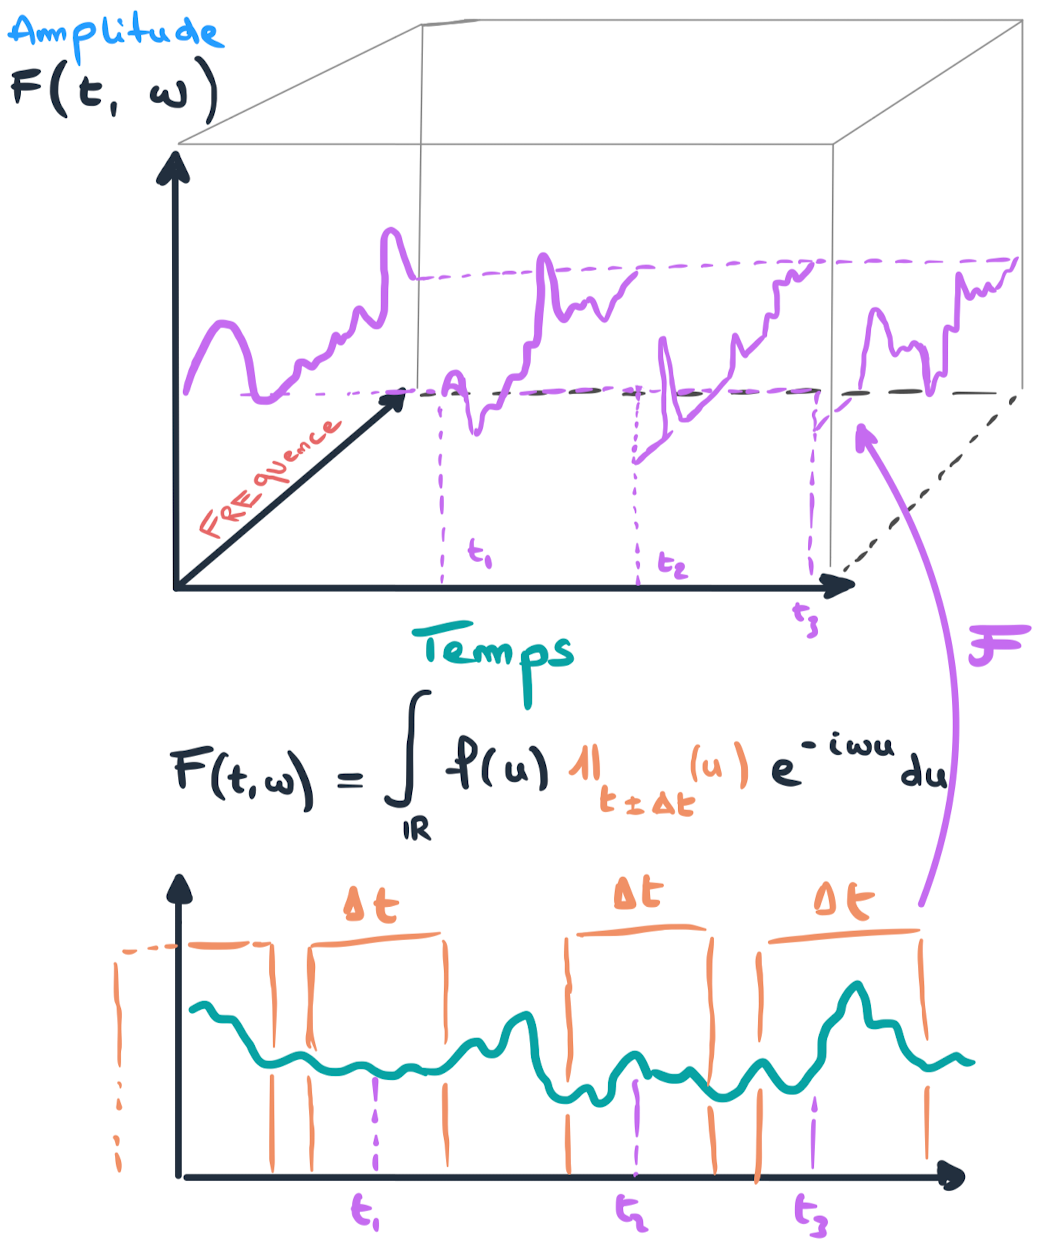
\includegraphics[width=\textwidth]{images/sketches/STFT.png}
		\caption{Transformée de Fourier à court terme d'une fonction}
		\label{fig:STFT}
	\end{figure}
\end{minipage}
\hfill
\begin{minipage}{0.60 \textwidth}

	Cependant contrairement à ce que peut suggérer le dessin présenté ici, la résolution fréquentielle n'est pas parfaite. Elle est d'ailleurs dans le cadre de la Transformée de Fourier à court terme constante, que ce soit sur le domaine temporel ou le domaine fréquentiel. La résolution fréquentielle est donc constante quelque soit la fréquence considérée.

	\question{
		\smallskip\centering
		Quel est le problème avec cette approche ?
	}

	le problème ne vient pas du monde mathématique mais plutôt du monde réel : les signaux que l'on observent présentent la caractéristique suivante : Les signaux de basse fréquence ont tendance à s'étendre sur la durée, et les signaux de hautes fréquences ont tendance à être très localisées, sous forme d'impulsion. Il devient alors clair que pour correctement identifier et localiser les fréquences présentes dans un signal, il est judicieux (voire parfois nécessaire) de varier la résolution fréquentielle et temporaire (limitées par le théorème d'indétermination de Heisenberg) en fonction de ce qui est le plus difficile à distinguer. C'est ce que proposent les ondelettes.

\end{minipage}

\subsubsection{Théorie de la base ondelettes}

\paragraph{Transformée en ondelettes}

Introduisons maintenant de façon plus formelle les ondelettes et regardons leurs propriétés intéressantes dans le cadre du lissage de trajectoires.

on définit la transformée en ondelettes vis à vis de l'ondelette mère $\psi$ d'une fonction $f$ par :

\begin{equation*}
	F : \begin{array}{ccc}
		\mathds R \times \mathds R_+ & \longrightarrow & \mathds R
		\\
		(t,s)                        & \longmapsto     & \displaystyle\frac 1 { \sqrt{|s|}} \int_{\mathds R} f(\colorize{u}) \psi \left( \frac{\colorize{u}-t}{s} \right) \mathrm d \colorize{u}
	\end{array}
\end{equation*}

\brain{on peut remarquer que la formule de la transformée en ondelettes ressemble à une projection : $\displaystyle\frac{\langle f, \psi_{t,s} \rangle_{\mathds L^2}}{|| \psi_{t,s} ||}$. Cela vient en quelque sorte motiver la section suivante}

\subparagraph{Base d'ondelettes}

\begin{minipage}{\linewidth}
	\begin{prop}[base d'ondelette dichotomique]
		\begin{equation*}
			\left\{ \psi_{k,n} : t \mapsto \frac 1 {\sqrt{2^k}} \psi\left( \frac{t - 2^k n}{2^k} \right) \right\}_{(k,n) \in \mathds Z^2} \textsf{ est une base } \vcenter{\hbox{$\underset{\| \cdot \|}{\perp}$}} \textsf{ de } \mathds L^2
		\end{equation*}
	\end{prop}
\end{minipage}


\info{notons que les résolutions sont des puissances de 2, ceci est un détail qui demandera une implémentation particulière dans le cadre des données réelles : il faudra faire attention à ce que le nombre de points que l'on donne dans l'algorithme de transformée rapide en ondelettes soit aussi une puissance de 2.}

\paragraph{Propriétés principales des ondelettes}

\smallskip


\subparagraph{Approximation dans l'espace fréquentiel-temporel}

La transofrmée en ondelettes
\begin{equation*}
	\mathcal W : f \mapsto \langle f \, | \, \psi_{t,s} \rangle
\end{equation*}
est une isométrie de $\mathds L^2$. Etant donné qu'elle est de plus une application linéaire, nous pouvons donc d'affirmer que

\begin{equation*}
	\boxed{|| f - \hat f ||_{\mathds L^2} = || \mathcal W f - \mathcal W \hat f ||_{\mathds L^2}}
\end{equation*}

Ainsi on peut travailler dans l'espace des ondelettes pour approximer (dans notre cas lisser les trajectoires) des fonctions et contrôler l'approximation directement dans le domaine fréquence-temporel tout en le conservant dans le domaine temporel.

\subparagraph{Propriété de Fast Decay : [ref : ~\cite{mallat-wavelet-course-ens-wavelet-zoom}]}

Une caractérisation des fonctions Hölderiennes, fournie par Antoniadis et Gijbels en 2002 \citationrequise est :

\begin{equation*}
	f \in \mathcal H_{\mathcal V(t_0)}(\alpha, L_\alpha) \cap \mathds L^2 \iff
	\begin{array}{l}
		\exists P \in \mathds R[X], \, \deg P \leq \alpha \leq \deg P + 1
		\\
		\exists f_{loc} \underset{t \rightarrow 0}{=} \mathcal O(t^\alpha)
	\end{array}
	\quad f(t_0 + h) \underset{t \rightarrow 0}{=} P(h) + f_{loc}(h)
\end{equation*}

\begin{definition}[vanishing moment]
	on dit qu'une ondelette $\psi$ possède $n$ vanishing-moments si :

	\begin{equation*}
		\forall k < n \prodscalselon{t \mapsto t^k}{\psi}{\mathds L^2} = 0 = \int_{\mathds R} t^k \psi(t) \, dt
	\end{equation*}

\end{definition}

\begin{prop}[vanishing-moment et polynômes]

\end{prop}

il suffit donc de choisir une ondelette avec $n > \alpha$ vanishing-moments pour obtenir :

\begin{equation*}
	\mathcal W f_{| \mathcal V(t_0)} {=} \mathcal W ( P + f_{loc} ) = \mathcal W P + \mathcal W f_{loc} = \mathcal W f_{loc}
\end{equation*}

enfin
\begin{thm}[Fast Decay | ref : ~\cite{mallat-wavelet-course-ens-wavelet-zoom} - thm 6.3]


	\begin{equation*}
		f \in \mathcal H_{\mathcal V({t_0})}(\alpha, L_\alpha) \cap \mathds L^2 \implies \exists A>0, \; \left|\left[\mathcal Wf\right](t, s)\right| \leq A \cdot s^{\alpha  + \frac 1 2}
	\end{equation*}

	et inversement en supposant $f$ bornée (ce qui est le cas pour une fonction continue sur un segment : notre cas) et $f$ Hölder juste après les bords. (C'est à dire que ça ne marche pas pour les points extrémaux $t \in \{0, 1\}$)
\end{thm}

Ainsi lorsque $s \in \left\{ 2^{-k} \right\}_{k \in \mathds N}$ :

\begin{equation*}
	\left|\left[\mathcal Wf\right](t, s)\right| \leq A \cdot 2^{-k(\alpha  + \frac 1 2)}
\end{equation*}

La magnitude de la transformée en ondelette décroit exponentiellement vers 0, et beaucoup plus rapidement là où $f$ est plus régulière. Ainsi, la transformée en ondelette agit comme un encodeur efficace d'information d'irrégularité




\subsubsection{Motivation dans le cadre de l'analyse de données fonctionnelles}

La capacité de capturer de façon efficiente les irrégularités de la fonction lissée est une motivation pour l'utilisation de la base d'ondelettes pour effectuer le pré-lissage de données, dont on espère qu'il n'écrase pas la majorité de l'information irrégulière de nos données. Si une des méthodes possibles, comme mentionnée précédemment, est d'utiliser un lissage non paramétrique à noyaux, les bases de fonctions ont de nombreux avantages. Un des avantage est le fait qu'une fois les projections sur la base déterminées, il n'y a plus besoin de se référer de nouveau aux données originales par la suite. Cela donne une représentation très parcimonieuse des données. Alors pour déterminer la valeur de $\widehat X(t)$ en un point $t$ non observé, il suffit d'évaluer l'expression $\sum_k \prodscal X {\psi_k} \psi_k(t)$.

\subsubsection{Effets du lissage à ondelettes sur la régularité locale}

\question{Peut on quantifier le biais introduit par le lissage en utilisant les ondelettes sur l'estimation de la régularité locale ?}

\editlater{regarder ce que ça donne, en utilisant les différents théorèmes et bornes disponibles sur les ondelettes pour un processus Holder LORSQUE J AI LE TEMPS - certainement en Septembre}


\subsection{Résumé de la méthodologie d'estimation de la régularité locale}

Résumons rapidement la méthode d'estimation de la régularité en un point $t_2 \in \mathcal T$.

\begin{figure}[H]
	\begin{center}
		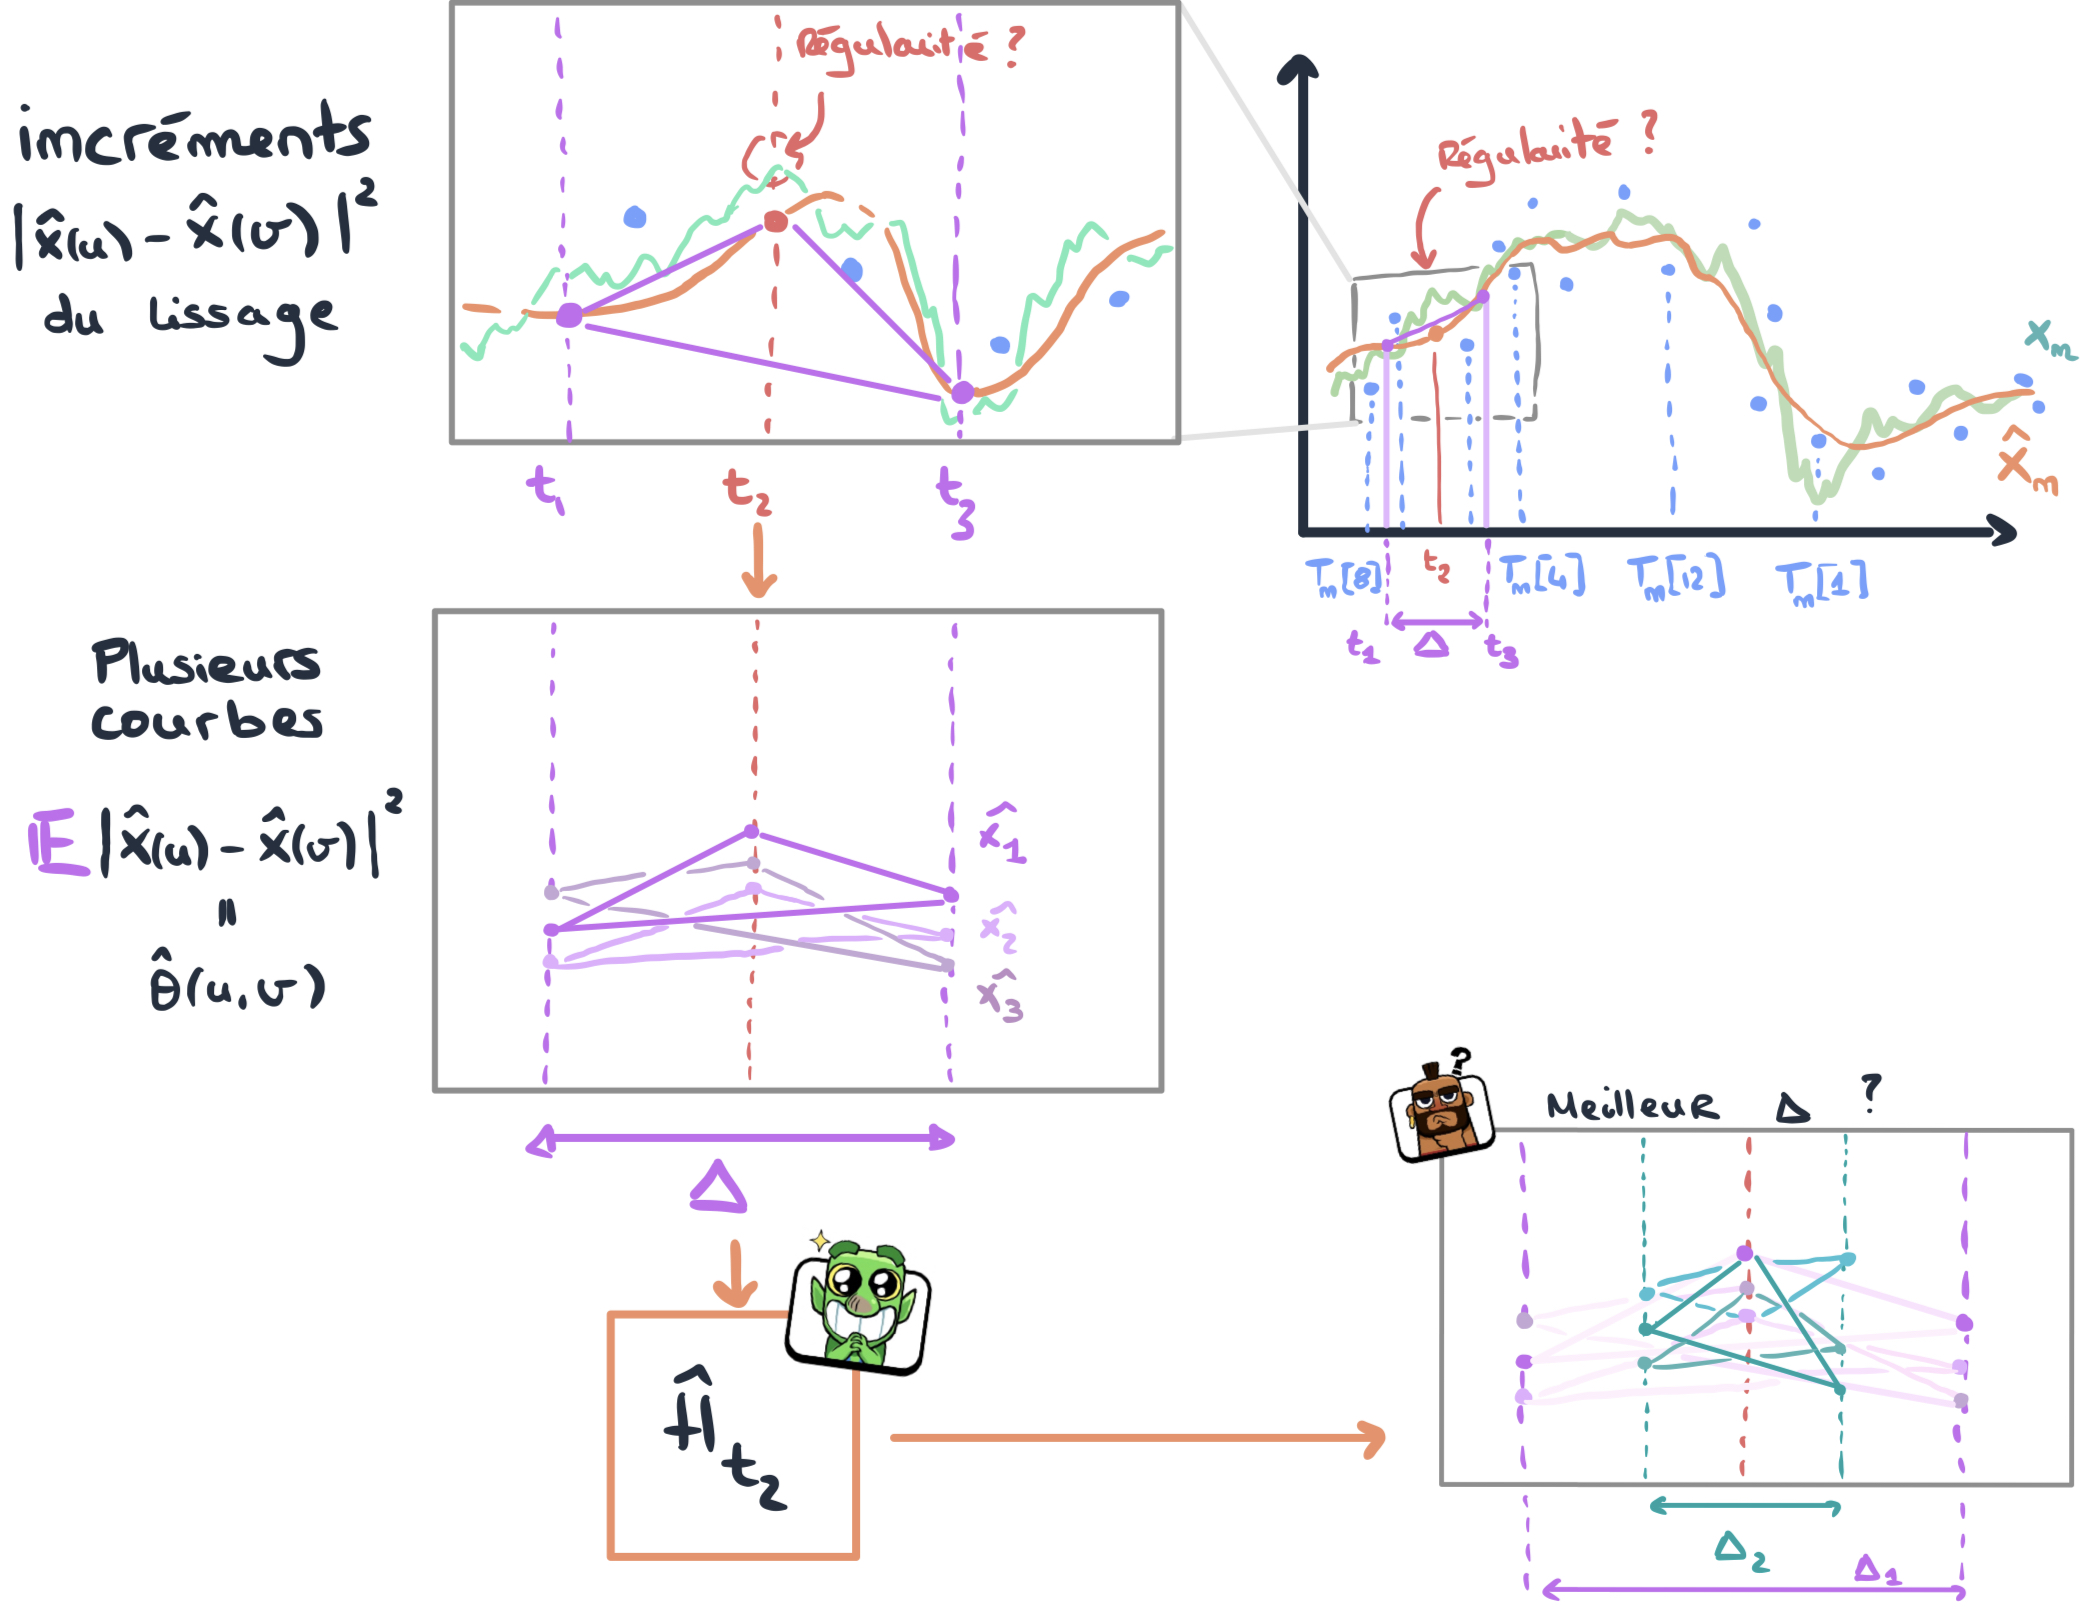
\includegraphics[width=\textwidth]{Images/sketches/estim_reg.jpg}
	\end{center}

	\caption{Schéma résumé de la méthode d'estimation de la régularité}
	\label{fig:sketch_estim_reg_methodo}
\end{figure}

La procédure d'obtention de la régularité est ainsi la suivante :

$\circled 1$ : Pré-lissage de la courbe

$\circled 2$ : Calcul des incréments quadratiques sur la courbe lissée

$\circled 3$ : moyennage des incréments (converge vers l'espérance sous hypothèse de dépendance faible)

$\circled 4$ : Utilisation de l'estimateur

Ce que nous cherchons désormais à déterminer est désormais la réponse à la question suivante :

\question{
	Quel $\Delta$ choisir pour obtenir la meilleure estimation de $H$ en $t_2$ ?
}

Pour étudier cela, nous allons simuler des données FAR(1) Höldériennes de régularité connue et allons étudier quel $\Delta$ fournit la meilleure estimation des paramètres de régularité en fonction de $\lambda$, $N$, $H_t$, ... \footnote{on pourra se référer à \ref{tab:model} pour la signification des notations}

